\documentclass{article}


\usepackage[utf8]{inputenc} %- Løser problem med å skrive andre enn engelske bokstaver f.eks æ,ø,å.
\usepackage[T1]{fontenc} %- Støtter koding av forskjellige fonter.
\usepackage{textcomp} % Støtter bruk av forskjellige fonter som dollartegn, copyright, en kvart, en halv mm, se http://gcp.fcaglp.unlp.edu.ar/_media/integrantes:psantamaria:latex:textcomp.pdf
\usepackage{csquotes}
\usepackage{url} % Gjør internett- og e-mail adresser klikkbare i tex-dokumentet.
\usepackage{hyperref} % Gjør referansene i tex-dokumentet klikkbare, slik at du kommer til referansen i referanselista.
\usepackage[norsk,english]{babel} % Ordbok. Hvis man setter norsk i options til usepackage babel kan man bruke norske ord.
\usepackage{amsmath} 				% Ekstra matematikkfunksjoner.
\usepackage{amssymb}
\usepackage{amsfonts}
\usepackage{amsthm}
\usepackage{mathrsfs}
\usepackage{mathtools}  
\usepackage{geometry}
\usepackage{tikz-cd}
\usepackage{graphicx}
\usepackage{svg}
\usepackage{changepage}
\usepackage{subcaption}
\usepackage{placeins}
\usepackage{bm}
\usepackage{physics}
\usepackage{siunitx}					% Må inkluderes for blant annet å få tilgang til kommandoen \SI (korrekte måltall med enheter)
  \sisetup{exponent-product = \cdot}      	% Prikk som multiplikasjonstegn (i steden for kryss).
   \sisetup{output-decimal-marker  =  {,}} 	% Komma som desimalskilletegn (i steden for punktum).
   \sisetup{separate-uncertainty = true}   	% Pluss-minus-form på usikkerhet (i steden for parentes). 
\usepackage{booktabs} % For å få tilgang til finere linjer (til bruk i tabeller og slikt).
\usepackage[font=small,labelfont=bf]{caption}		% For justering av figurtekst og tabelltekst.
\usepackage[
backend=biber,
]{biblatex}
\addbibresource{ref.bib}

% math stuff
\newcommand{\restr}[2]{\ensuremath{\left.#1\right|_{#2}}}

% my personal commands
\newcommand{\R}{\mathbb{R}}

%\clearpage % Bruk denne kommandoen dersom du vil ha ny side etter det er satt plass til figuren.
% Disse kommandoene kan gjøre det enklere for LaTeX å plassere figurer og tabeller der du ønsker.
\setcounter{totalnumber}{5}
\renewcommand{\textfraction}{0.05}
\renewcommand{\topfraction}{0.95}
\renewcommand{\bottomfraction}{0.95}
\renewcommand{\floatpagefraction}{0.35}

% math stuff

\newtheorem{definition}{Definition}[section]
\newtheorem{theorem}{Theorem}[section]
\newtheorem{claim}[theorem]{Claim}
\newtheorem{proposition}[theorem]{Proposition}
\newtheorem{lemma}[theorem]{Lemma}
\newtheorem{corollary}[theorem]{Corollary}
\newtheorem{conjecture}[theorem]{Conjecture}
\newtheorem*{observation}{Observation}
\newtheorem*{example}{Example}
\newtheorem*{remark}{Remark}

\usepackage{bbm}
\newcommand{\DiffI}{\text{Diff}^+(I)}
\newcommand{\Diffp}{\text{Diff}^+}
\newcommand{\id}{\text{id}}
\newcommand{\one}{\mathbbm{1}}

\graphicspath{{..}}
\addbibresource{ref.bib}

\title{Specialization Project}

\author{Alexander Johan Arntzen }

\date{\today}
%%%%%%%%%%%%%%%%%%%%%%%%%%%%%%%%%%%%%%%%%%%%%%%%%%%%%%%%%%%%%%%%%%%%%%%%%
\begin{document}

\maketitle
\tableofcontents

\section{Introduction}
\todo{introduce shape analysis and SRVT}
\todo{applications, optimization problem}
\todo{introdue optimizion with neural networks}
The neural network optimization procedure will then be compared to a similar gradient-based and dynamic programming algorithm.
% 
\section{Theory}
\subsection{Riemannian manifolds}
Define riemannian metric
\subsection{Lie groups}
this subsection some basic Lie group properties are introduced. Based on \cite{celledoni2016}. Basic knowledge of smooth manifolds is assumed.
\begin{definition}[Lie group]
  A Lie group  \(G\) is a smooth manifold that is also a group, such that multiplication
  \begin{equation}
    \mu : G \times G \rightarrow G
  \end{equation}
  and inversion
  \begin{equation}
    i : G  \rightarrow G
  \end{equation}
  are smooth.
\end{definition}
Since both  multiplication and inversion are smooth we define multiplication by  \(g \in G\) as diffeomorphism.
\begin{definition}
  Let  \(G\) be a Lie group and  \(g \in G\). Then the \textbf{right translation} by  \(g\) is defined as
  \begin{equation}
    R_g(h):= hg \quad  \forall \ h  \in G.
  \end{equation}
\end{definition}
\begin{remark}
  in this text we use the \textbf{right} translation, but we could similarly define the left translation.
\end{remark}
Once translation is defined, the following property of vector fields follows.
\begin{definition}
  A vector field  \(X\) on a Lie group  \(G\) is \textbf{right invariant} if it is invariant under the pushforward of all right translation. That is is
  \begin{equation}
    (r_g)_*X = X  \quad \forall g \in G
  \end{equation}
\end{definition}
An invariant vector field  \(X\) on a Lie group  \(G\) is thus uniquely defined by the vector field's value at the identity element  \(e\). Similarly, for all vectors  \(\xi \in T_eG\) we can define an invariant vector field   \(X^{\xi}\) on  \(G\).
\begin{definition}[Lie algebra]
  Let  \(e\) be the identity element of the Lie group  \(G\). Then the \textbf{Lie algebra}  \(\mathfrak{g}\) is the vector space  \(T_{e}G\) together with a lie bracket as bilinear product.
\end{definition}
\subsection{The exponential map}

\begin{definition}[Exponential map]
  Let  \(\mathfrak{g}\) be the Lie algebra of the Lie group  \(G\) with identity  \(e\). For all  \(\xi \in \mathfrak{g}\) let  \(\gamma^{\xi}\) be the integral curve of the right invariant vector field  \(X^{\xi}\) where  \(X^\xi (e)=\xi\) and  \(\gamma^\xi(0) = e\). The \textbf{exponential map} is the map  \(\exp : \mathfrak{g} \rightarrow G\) such that  \(\exp(\xi) = \gamma^\xi(1)\).
\end{definition}
% TODO: make an argumet for why it is well defined
\begin{proposition}
  Let  \(X\) be a right invariant vector field on the Lie group  \(G\) with identity  \(e\). Then the flow of  \(X\),  \(\phi_t\) is given by  \(\phi_t(g) = \exp(tX(e))g\) for all  \(g\) in  \(G\).
\end{proposition}
\begin{proof}
  Denote  \(\gamma^{\xi}\) as the integral curve of an  invariant vector field  \(X^{\xi}\)such that  \(\dot{\gamma}^{\xi}(0) = \xi\) and  \(\gamma^\xi(0)=e\). Then  \(\gamma^{t\xi}(0) =  \gamma^{\xi}(0)=e\) and
  \begin{equation}
    \frac{d}{ds}\gamma^{\xi}(ts) = t\dot\gamma^{\xi}(st)=tX^\xi(\gamma^{\xi}(ts)) = t D R_{\gamma^\xi(ts)} \vert_{e} \xi = X^{t\xi}(\gamma^{\xi}(ts)).
  \end{equation}
  So  \(\gamma^\xi(ts)\) is the integral curve of  \(X^{t\xi}\) and  \(\gamma^\xi(ts)=\gamma^{t\xi}(s)\). Therefore,   \(\exp(t\xi) = \gamma^{\xi}(t)\).

  Now, we can show that  \(\exp(tX(e))g\) is the integral curve of  \(X^{\xi}\) starting at  \(g\). Firstly,  \(\exp(0)g = \gamma^{t\xi}(0)g=g\). Then, computing the derivative we have
  \begin{equation}
    \frac{d}{dt} \exp(t\xi)g = D R_g \vert_{\gamma^\xi(t)} X^\xi(\gamma^\xi(t)) = X^\xi(\exp(t\xi)g).
  \end{equation}
  By uniqueness of integral curves the result follows.
\end{proof}
% TODO: show that the flow is defined for all times t 
\begin{remark}
  If  \(G\) is a subgroup of  \(GL(n)\) then it can be shown that the  \(\exp(A)\) is the matrix exponential  \(e^{A}\).
\end{remark}


The exponential map also has a unique inverse in a neigboorhodd.
\begin{definition}[Logatimic derivative]
  \(\delta^r(\gamma)\)
\end{definition}
\begin{proposition}
  The right logarithmic derivative is the inverse of the exponential map?
\end{proposition}

\section{Shape analysis}
\subsection{Definitions and motivation}
To start the problem of analyzing curves we fist introduce the space of curves that are considered in this project. We will follow the approxach given by \citeauthor[]{bauer2015why} in \cite{bauer2015why}. The curves we will consider will be the space of all immersions from the interval  \(I = [0, 1]\) to  \(\R^d\)
\begin{equation}
  \mathcal{P}:= \text{Imm}(I, \R^d) = \{c \in C^{\infty}(I, \R^d) :  c'(t) \neq  0 \ \forall \ t \in I  \}.
\end{equation}
The space \(\mathcal{P}\) is genrally called the \emph{pre-shape space}. Analysis of closed curves \(\text{Imm}(S^1, \R^d)\) and surfaces \(\text{Imm}(I \times I, \R^d)\) can also be done within a simmilar framework \cite{bauer2014overview}.
The following can also be applied to immersions into other spaces than \(\R^d\). This, will be the content of section\ref{subsec:shape-lie}. 

Now we would like to study shapes independent of parametrization. More precisely, the space af all curve reparametrizations   \(\varphi\) is the group of orientation preserving diffeomorphisms on  \(I\)
\begin{equation}
  \text{Diff}^+(I) = \{\varphi \in C^{\infty}(I,I): \varphi(0) = 0, \varphi(1) = 1, \varphi'(t) > 0 \ \forall \ t \in I \}.
\end{equation}
Furthermore, for a reparametrization  \(\varphi \) and a curve  \(c\)a group action can be defined by  \(c \circ \varphi\). Thus we can define the space of parameterized curves \(\mathcal{S}\) as the quotient space under this group action,
\begin{equation}
  \mathcal{S} := \mathcal{P} \ / \ {\text{Diff}^+(I)}.
\end{equation}
The space  \(\mathcal{S}\) is called the \emph{shape space} an with elements called \emph{shapes}. Furthermore, the space \(\mathcal{S}\) is iteself a infinite dimentional manifold with the projection map beeing a submersion. 

\subsection{Distance on shape space}
To find a distance function \(d_{\mathcal{S}}\) on \(\mathcal{S}\) we start with distance on \(\mathcal{\mathcal{P}}\) that is \emph{reparametrization invariant}. That is, \(d_\mathcal{P} : \mathcal{P} \times P \rightarrow (0, \infty)\) has the property that for all  \(c_1, c_2 \in \mathcal{P}\)
\begin{equation}
  d_{\mathcal{P}}(c_1, c_2)=d_{\mathcal{P}}(c_1 \circ \varphi, c_2\circ \varphi) \quad \forall \varphi \in \text{Diff}^+.
\end{equation}

A reparametrization invariant distance funcition on \(\mathcal{P}\) will not nessearly be a distance function on \(S\) since  that distance between representatives of each shape has to be the same. Thus, a distance function on \(\mathcal{S}\) will we defined as. 
\begin{equation}
  d_\mathcal{S} ([c_1],[c_2]) := \inf_{\varphi \in \text{Diff}^+}{  d_{\mathcal{P}}(c_1,c_2 \circ \varphi)},
  \label{eq:distance_inf}
\end{equation} 
where  \([c_1]\) and  \([c_2]\) are the shapes with reparametrizations \(c_1\) and  \(c_2\). 

\subsection{Rimannian metric on shape space}
As remarked note in \cite{bauer2014overview} the the shape space \(\mathcal{S}\) inherently non-linear. Therefore we impose a \emph{reparametrization invariant Rimannian metric}  on \(\mathcal{P}\). That is, a metric \(G\) such that for all \( c \in \mathcal{P}\) and \(h,k \in C^\infty\)
\begin{equation}
  G_c(h,k) = G_{c \circ \varphi}(h\circ \varphi, k \circ \varphi) \quad \forall \varphi \in \text{Diff}^+.
\end{equation}
A reparametrization invariant Riemannian metric will then induce a reparametrization invariant induced geodesic distance given by 
\begin{equation}
  d_\mathcal{P}(c_1, c_2) = \inf_{
    \substack{
      \gamma \in C^{\infty}([0,1], \mathcal{P}) \\ 
      \gamma(0) = c_1 \\
      \gamma(1) = c_2
    }
  } \int_0^1 \sqrt{G_{\gamma(t)}(\gamma'(t),\gamma'(t))} \, dt.
\end{equation}
A distance function on \(\mathcal{S}\) can then be obtained by \eqref{eq:distance_inf}. The Rimannian metric on \(\mathcal{P}\) also defines a unique Rimannian metric on \(\mathcal{S}\) such that the projection map from \(\mathcal{P}\)  to \(\mathcal{S}\) is a Rimannian submersion \cite[6]{bruveris1016_srvtexample}. 

An obvious metric on \(\mathcal{P}\) is the \(L^2\) metric  given by 
\begin{equation}
  G_c(h,k) = \int_I \langle h, k\rangle \vert c'\vert \,dt. 
\end{equation}
However as shown in \cite{michor2003vanishingl2} and \cite{michor2004vanishing_generalized} the \(L^2\) metric induces a vanishing distance on shape space \(\mathcal{S}\). This means that for any \(c_1, c_2 \in \mathcal{P}\) we can curves \(\gamma \in C^{\infty}([0,1],\mathcal{P})\) starting at \(c_1\) ending at \(c_2\) of arbitrary short length. As a consclusin the \(L^2\) metric is useless for comparing shapes, and so we must find another metric. 

\subsection{Square root velocity transform}
A method for imposig a metric on \(\mathcal{P}\) is to transform the curves with a diffeomorphism to another Riemannian manifold resulting in a pullback metric on \(\mathcal{P}\). A popular such transformation introduced in \cite{srivastava2011_srvt} is the \emph{sqare root velocity transform} (SRVT), wich is given by 
\begin{equation}\label{eq:SRVT}
  R :\mathcal{P} \rightarrow C^{\infty}(I, R^d \setminus \{0\}), \quad c \mapsto \frac{c'}{\sqrt{\vert c' \vert}}.
\end{equation} 

The SRVT has several properies wich is not proved here; for a thoroguh  see \cite{bruveris1016_srvtexample,bauer2014_rprop}. Firstly, as stated in equation \eqref{eq:SRVT} the SRVT is not injective, since it invariant under translation. It will however, be a diffeomorphism between the space of curves with zero starting position \(\mathcal{P}_* : = \{c \in \mathcal{P}: c(0) = 0\} \) and \(C^{\infty}(I, \R^d \setminus \{0\}\) with an analytical inverse on the form 
\begin{equation}
  R^{-1}(q)(t) = \int_0 ^t q \vert q\vert \,d\tau.
\end{equation}
Furthermore, imposing the \(L^2\) inner product on\((C^{\infty}(I, R^d), \langle \cdot , \cdot \rangle_{L^2} )\) gives an inner product space. Thus, the SRVT imposes a pullback distance metric and riemanninan metric on \(\mathcal{P}_*\). The pullback distance metric for the two curves \(c_1, c_2 \in \mathcal{P}_*\) will be given by
\begin{equation}\label{eq:sob_pullback_dist}
  d_{\mathcal{P}_*}(c_1, c_2) = \norm{R(c_1) - R(c_2)}_{L^2}.
\end{equation}
Similarly, the pullback Riemannian metric on \(\mathcal{P}_*\) will be an \emph{first order Sobolev metric} defined by the arch length integral
\begin{equation}
  G_c(h,k) = \int_I \langle D_s h^\perp ,D_s^\perp k \rangle+\frac{1}{4}\langle D_s h,v\rangle \langle D_s k,v\rangle \,ds,
\end{equation}
where \(ds = \vert c' \vert\,dt\), \(v = D_s c = \frac{c'}{\vert c'\vert}\) is the curve of unit length tangents of \(c\) and \(D_s h \perp = D_s h  - \langle D_s h,v\rangle v\) is the projection of \(D_s h\) onto the space of curves orhtognal to \(v\). \todo{remark on properties of this metric}

The space \(C^{\infty}(I, \R^d \setminus \{0\} \) is flat, but not convex. Therefore, when the SRVT of any two curves \(R(c_1), R(c_2)\) belong to the same convex subset of \(C^{\infty}(I, \R^d \setminus \{0\})\). Then the  godecis from \(c_1\) to \(c_2\) is given by 
\begin{equation}
  \gamma(t) = R^{-1}[R(c_2)t +  R(c_1)(1-t)], 
\end{equation}
and geodesic distance corresponds to the metric \(d_{\mathcal{P}_*}\). For transformed curves not connected by a straight line there are two cases. Either the geodesic of the metric \(G\) will not exist, or the geodesic distance induced by \(G\) will not correspond to the  distance \(d_{\mathcal{P}_*}\). When \(d \geq 3\),  we can make lines in \(C^{\infty}(I, \R^d )\) into paths in \(C^{\infty}(I, \R^d \setminus \{0\}\) by arbitrary small pertubations. Thus, the distance given by \(d_{\mathcal{P}_*}\) will be the induced geodesic distanc of \(G\). As a remedy for \(d \leq 2 \), it is possible to consider geodesic completions of \(\mathcal{P}_* \) as discussed in \cite{bruveris1016_srvtexample} and more generally in \cite{bruveris2014_geocomp}. 


To extent the Riemannian geometry of to the shape space we note that the SRVT has the equivariance property: 
\begin{equation}
  R(c \circ \varphi) = \sqrt{\varphi'}R(c) \circ \varphi \quad \forall \ \varphi \in \text{Diff}^+, c \in \mathcal{P}. 
\end{equation}
Therefore, we deduce by integration or \cite[Theomrem 3.1]{bauer2014_rprop} that the metrics \(G\) and \(d_{\mathcal{P}_*}\) are reparametrization invariant. The reparametrization invariant metrics can then be extended to \(\mathcal{S}_* : =  \{[c] \in \mathcal{S}: c(0)=0\}\) by \eqref{eq:distance_inf}. For finding distances and geodesics between two shapes \([c_1], [c_2]\in \mathcal{S}_*\) we need to find a reparametrization \(\varphi \in \DiffI\) that minimizes 
\begin{equation} \label{eq:srvt_reparam}
  \norm{R(c_1) - \sqrt{\varphi'} R(c_2)\circ \varphi}_{L^2}. 
\end{equation}

The optimal solution to the optimization problem above will not nessearly exist in \(\DiffI\). For examples of curves that lead to optimal reparametrization outside \(\DiffI\) see \cite[p.11]{bauer2014overview} and \cite[3.2]{woien2019}. One problem is that optimal solutions  have vanishing derrivatives. Thus the optimal solution is not a diffeomorphism and does not have a inverse. \citeauthor{bruveris1016_srvtexample} \cite{bruveris1016_srvtexample}  remidies this problem by showing that for curves \(c_1, c_2 \in C^2(I,\R^d\) there exists optimal reparametrizations \(\varphi_1^*, \varphi_2^* \in \overline{ \Gamma}\) that minimizes
\begin{equation}
  d_{\mathcal{P}_*}(c_1 \circ \varphi_1, c_2 \circ \varphi2). 
\end{equation}
The space of reparametrizations is now extened to 
\begin{equation}
  \overline \Gamma = \{\gamma : I \rightarrow I : \gamma \text{abs. cont. }, \gamma(0) = 0, \gamma(1) = 1, \gamma' \geq 0 \text{a.e.}\}.
\end{equation}

\subsection{Shape analysis on Lie groups}\label{subsec:shape-lie}
In \cite{celledoni2016} an extension of the SRVT to Lie groups is intrudoces. 
Reparametrization equivarint 
\todo{definins and commetns}
\todo{motion capture data}

\section{Optimal reparametrization}
\subsection{Problem }
\subsection{Discretization}

\subsection{Dynamic programing}
\subsection{Deep reparametrization}

\section{Reparametrization with neural networks}
This section introduces a method to find the optimal reparametrization using neural networks. It was inspired by \citeauthor{jørgen2021}'s deep reparametrization method \cite{jørgen2021}. In deep reparametrization, solutions are constructed much like a residual neural network. Consequently, modeling reparametrizations as neural networks is a natural choice.

\subsection{Feedforward Neural networks}
Neural networks have been used successfully in many different fields and come in many different forms. Furthermore, there are multiple ways of defining neural networks and many different universal approximation results. We define neural networks similarly to \cite{cybenko1989} by first defining the following nonlinearity property.
\begin{definition}[Sigmoidal function]
  A sigmoidal function is a function \(\sigma : \R \rightarrow \R \) such that
  \begin{equation*}
    \lim_{t \rightarrow \infty}\sigma(t) = 1 \quad \and \text{and} \quad  \lim_{t \rightarrow -\infty}\sigma(t) = 0.
  \end{equation*}
\end{definition}
We then define feedforward neural networks as follows.
\begin{definition}[Feedforward Neural Networks]
  For a sigmoidal function \(\sigma\), a \emph{feedforward neural network} is a function on the form
  \begin{equation*}
    f_\theta  = A_L \circ \sigma \circ A_{L-1} \circ \sigma \cdots  \sigma \circ A_1,
  \end{equation*}
  where \(\sigma\) is applied componentwise and \(\theta = {(W_k, b_k)}_{k = 1}^L\) determines the affine functions \(A_k: \R^{l_{k-1}} \rightarrow \R^{l_k} : x \mapsto W_k x + b_k \). \todo{parameter space \(\Theta\)}
\end{definition}
\begin{remark}
  There are several naming conventions on the parameters of neural networks. The parameter \(L\) denotes the number of layers or \emph{depth}, and \(L-1\) is the number of \emph{hidden} layers. Also for each layer, \(l_k\) is called the \emph{width} of the layer. Neural networks with one hidden layer are called \emph{shallow}. Similarly, networks with more hidden layers \(L > 2\) are called \emph{deep}.
\end{remark}

An important property of neural networks is that they are universal approximators. More concretely, a classical result \cite[Theorem 2]{cybenko1989} states that the space of all shallow feedforward neural networks with a continuous sigmoidal are dense in \(C(I_n)\), where \(C(I_n)\) is the banach space of continuous functions from the unit cube in \(\R^n\) with the infinity norm.  Furthermore, for a specific sigmoidal function, it is possible to prove an estimate of how the necessary width and depth of feedforward networks grows with increasing approximation error. Specifically, with the \(\tanh\) sigmoidal function \citeauthor{ryck2021} \cite[Theorem 5.1]{ryck2021} show that for all \(\epsilon > 0 \) and \(f \in C^k(I_n)\). There exist a network \(\hat{f_\epsilon}\) with width \(\mathcal{O}(\epsilon^{n / k})\) such that
\begin{equation*}
  \norm{f - \hat{f_\epsilon}}_\infty < \epsilon.
\end{equation*}
For networks with ReLu sigmoidal functions, similar estimates have been proven by \citeauthor{yarotsky2017} \cite{yarotsky2017}. Thus, we conclude that it is possible to approximate diffeomorphisms of \(I\)  with neural networks.

\todo{comment on automatic differentiation}

\subsection{Neural networks as reparametrizations}\label{subsec:neural-nets}
Reparametrization using neural networks is based on four ideas. Firstly, neural networks approximate any reparametrization in \(\DiffI\) arbitrarily well. Secondly, using a quadrature rule as in \eqref{eq:discretized_cost}, we end up with a cost function \(\hat E(\theta)\) which consistently approximates the true error \(E(f_\theta)\). The optimal reparametrization can then be found by optimizing \(\hat E\) with a gradient-based algorithm like BFGS\@. Finally, we need to ensure that the final solution belongs to \(\DiffI\).

A solution \(f_\theta : \R \rightarrow \R \) must fulfill three constrains to be a in \(\DiffI \). The first one, smoothness, is achieved by selecting a smooth sigmoidal function. The boundary conditions and positiveness of \(f_\theta'\) are then enforced by adding penalizing terms to the cost function. The new cost function will therefore need to minimize the following therms
\begin{align*}
  \mathcal{K}_{\text{int},\theta}(t)  & = q_1(t) - \sqrt{\dot f_\theta(t)}q_2 \circ f_\theta(t), \\
  \mathcal{K}_{\text{Diff},\theta}(t) & = \one_{(-\infty,0]}\dot f_{\theta}(t),                  \\
  \mathcal{K}_{b,\theta}              & = \abs{f_\theta(0)}^2 + \abs{f_\theta(1) - 1}^2.
\end{align*}
There is no obvious relation between the sizes of the three penalties. Therefore, the new cost function will be their weighted sum
\begin{equation}\label{eq:neural_cost}
  \mathcal{J}(\theta) =
  \frac{1}{N}\sum_{i=n}^{N_i}{
  \big(
  w_\text{int}\abs{\mathcal{K}_{\text{int},\theta}(t_i)}^2 +
  w_{\text{Diff}}|{\mathcal{K}}_{\text{Diff}, \theta}(t_i)|^2
  \big)} +
  w_{b}{\mathcal{K}}_{b,\theta} +
  \lambda||\theta||_2,
\end{equation}
where  \(w_\text{int}, w_{b} \) and  \(w_{\text{Diff}}\) are parameters penalizing each residual. Furthermore, \(\lambda\) is a regularization parameter where \(\theta\) is treated as vector.

\subsection{Discontinuous SRV form}\label{subsec:discont_curves}
Optimizing the new cost function \(\mathcal{J}\) will not necessarily work for curves that have a discontinuous SRV form \(q_1, q_2\). If one of the transformed curves is discontinuous, there is no guarantee that the cost function will be continuous. The discontinuous optimization problem will be harder to solve and can not be solved with a typical gradient-based method.

A general theory of when discontinuous curves results in a discontinuous cost function will not be attempted. Instead we look at a situation when the the cost function is guaranteed to be discontinuous at a point \(\theta_0\). Consider a transformed curve  \(r\) that is discontinuous at  \(a \in I\). Moreover, assume that the reparametrizations  \(f_{\theta}\) is smooth with respect to the parameters  \(\theta\), \(f_{\theta_0}(t')=a\) and  \(\pdv{f}{\theta_1}|_{\theta_0}(t')\neq 0\) for some  \(\theta_0\) and direction \(\theta_1\). Then along the direction  \(\theta_1\),  \(f_{\theta}\) will have a a continuous inverse in some neighborhood  \(N\) of  \(\theta_0\). Thus, since \(\sqrt{f_{\theta}'(t')} \geq 0\), \(r \circ f_\theta(t')\) and  \(\sqrt{f_{\theta}'(t')} r \circ f_\theta(t')\) will be discontinuous at \(\theta_0\). If we then assume that
\begin{equation*}
  \sqrt{f_{\theta}'(t')} r \circ f_\theta(t') \geq  q(t')\ \text{on} \ N,
\end{equation*}
or
\begin{equation*}
  \sqrt{f_{\theta}'(t')} r \circ f_\theta(t') \leq q(t') \ \text{on} \ N.
\end{equation*}
Then the cost function defined as
\begin{equation*}
  E_0(\theta) = \big[q(t') - \sqrt{f'_{\theta}} r \circ f_{\theta}(t')\big]^2,
\end{equation*}
will have a discontinuity at  \(\theta_0\). The cost function as defined in \eqref{eq:neural_cost} will then be discontinuous if the discontinuities in each part of the sum does not cancel each other.

The assumptions required of  \(f_{\theta}\) are not necessary for \(E_0\) to be discontinuous. It is only a reasonable situation where \(E_0\) is guaranteed to be discontinuous.

For transformed curves that are not continuous, there is a way to find an approximate solution to the optimal reparametrization problem. If the jumps of the discontinuous curve \(r\) are not too large, then we can use a new continuous curve \(\hat r\) that interpolates \(r\). Then, we can find a bound for the error resulting from using the continuous curve instead of the discontinuous one to calculate distances. The following proposition specifies this bound.
\begin{proposition}\label{prop:distance_difference}
  Let \({\{t_i\}}_{1 \leq i\leq n}\) be a strictly increasing sequence of numbers in the interval I, and let \(q\),\(r\), \(\hat q\) and  \(\hat r\) curves such that \(q(s_i)=\hat q(s_i)\) and \(r(s_i')=\hat r(s_i')\) for \(s_i, s_i' \in [t_i, t_i+1), 1\leq i < n\). If  \(q\),  \(r\),   \(\hat q\) and  \(\hat r\) are smooth on the intervals  \([t_i, t_{i+1})\) for  \( 1 \leq i <n\), and  \(f_\theta : I \rightarrow I\) is a function with bounded derivative and parametrized by \( \theta \). Then the difference between the distances
  \begin{align*}
    \hat d_n^2=\frac{1}{n}\sum_{i=1}^{n}\Big|\hat q(t_i) + \sqrt{f'_{\theta}(t_0)} \hat r \circ f_{\theta}(t_0)\Big|^2, \\
    d_n^2=\frac{1}{n}\sum_{i=1}^{n}\Big|q(t_i) + \sqrt{f'_{\theta}(t_0)} r \circ f_{\theta}(t_0)\Big|^2,
  \end{align*}
  is bounded by
  \begin{equation*}
    | \hat d_n -d_n | \leq  C h,
  \end{equation*}
  where h = \(\max_{1\leq i<n}|t_{i+1} - t_{i} |\), and C is a constant depending on the derivatives of  \(r\),  \(\hat{r}\),  \(q\),  \(\hat q\) and  \(f_{\theta}\).
\end{proposition}
\begin{proof}
  On  \([t_i, t_{i+1})\),  \(\hat q\) and  \(\hat r\) are smooth functions that are equal to  \(q\) and  \(r\) in a point  \(t' \in [t_i, t_{i+1})\). Thus by Taylor's theorem for all  \(t \in [t_i, t_{i+1})\) there exist  \(\xi \in (t_i, t_{i+1})\) such that
  \begin{align*}
    |\hat q(t) - q(t)| & = |\hat q'(\xi) - q'(\xi)||t' - t|  \\
    |\hat r(t) - r(t)| & = |\hat r'(\xi) - r'(\xi)||t' - t|.
  \end{align*}
  Now define  \(T:= \left \{t_i : 1 \leq i \leq n \right \} \). Then, since all  \(t \in I\) are in some interval of length  \(h\) we have to following bounds
  \begin{align*}
    ||\hat q - q||_{\infty} \leq ||\hat q' - q'||_{\infty, I \setminus T}h = C_q h,
  \end{align*}
  \begin{align*}
    ||\hat r - r||_{\infty} \leq ||\hat r' - r'||_{\infty, I \setminus T}h = C_r h.
  \end{align*}
  Now define constant  \(C_{\theta}:= \sup_{t\in T} | \sqrt{f'_\theta(t)} | \). Then by the reverse triangle inequality for the 2-norm we have the bound
  \begin{align*}
    |\hat d_n - d_n |
     & = \Bigg| \sqrt{\frac{1}{n}\sum_{i=1}^{n}\Big|\hat q(t_i) + \sqrt{f'_{\theta}(t_0)} \hat r \circ f_{\theta}(t_0)\Big|^2}-\sqrt{\frac{1}{n}\sum_{i=1}^{n}\Big|q(t_i) + \sqrt{f'_{\theta}(t_0)} r \circ f_{\theta}(t_0)\Big|^2 } \Bigg| \\
     & \leq \sqrt{\frac{1}{n}\sum_{i=1}^{n}\Big|\hat q(t_i) - q(t_i)  + \sqrt{f'_{\theta}(t_i)}\left[  \hat r \circ f_{\theta}(t_i) - r \circ f_{\theta}(t_i)\right]\Big|^2}                                                                \\
     & \leq \left(C_q  + C_{\theta} C_r \right)h.
  \end{align*}
\end{proof}

As a consequence, if we have two smooth curves with piecewise constant interplants \(r, q\) that results in the cost function \(E\) defined as in \eqref{eq:discretized_cost}. If we also construct a continuous and piecewise linear function \(\hat r\) interpolating \(r\) at \(\{t_i\}, 1 \leq i <n\). Then, replacing \(r\) by \(\hat r\) results in cost function  \(\hat{E}\) such that \(|\hat{E} - E |= \mathcal{O}(1/n)\).


As seen in chapter \ref{subsec:shape-lie} motion capture data can be viewed as a smooth curve in \({SO(3)}^m\). If this motion is record at at discrete times, then the resulting geodesic interpolation results in a SRVT that is piecewise constant. Thus for two motions, we have two smooth curves with piecewise constant interpolations \(q_1, q_2\) in SRV form. The optimal parametrization problem results in the cost discontinuous function\(E\). If we then construct a continuous piecewise linear function \(\hat r\) interpolating \(r\) at \(\{t_i\}, 1 \leq i <n\). Then replacing \(r\) by \(\hat r\) results in cost function  \(\hat{E}\) such that \(|\hat{E} - E |= \mathcal{O}(1/n)\).

\FloatBarrier

\section{Experiments}
\FloatBarrier
When dealing with neural networks there are a wide range of network structures and optimization algorithms. An in depth search for the best parameters will not be the focus of this chapter. The main focus of this chapter will be to investigate when reparametrization by neural networks is possible.

We also investigate whether the deviation from the optimal solution is optimization error or approximation error.  Thus by the results in chapter [0] we investigate how increasing the network size impacts the resulting error. This approach will still be somewhat ambiguous; since increasing the networks size simultaneously increases the dimension of the optimization problem. Also with increasing layers we have the vanishing gradient problem.[0]

\subsection{Curves from the same shape}
\FloatBarrier
In this experiment we used the example from \cite[Section 4.2.6]{jørgen2021}. The SRVT was not used in the original experiment, but SRV form of the two curves considered are the same. Thus, we considered a curve with SRV form \(r\) given by 
\begin{equation*}
    r(t) = \pi [-2 \sin(2\pi t), 4\cos(4\pi t)]^T,
\end{equation*}
and its reparametrization \(q = \sqrt{\psi'}q \circ \psi\), where 
\begin{equation*}
    \psi(t) = \frac{\log(20t + 1)}{2 \log(21)} + \frac{\tanh(20(t - 0.5))}{4 \tanh(10)}.
\end{equation*}
The SRV form of the curves is shown in Figure \ref{fig:curve_1}. 

\begin{figure}[b]
    % \begin{subfigure}[b]{0.5\textwidth}\label{fig:curve_1_c_1}
    %     \centering
    %     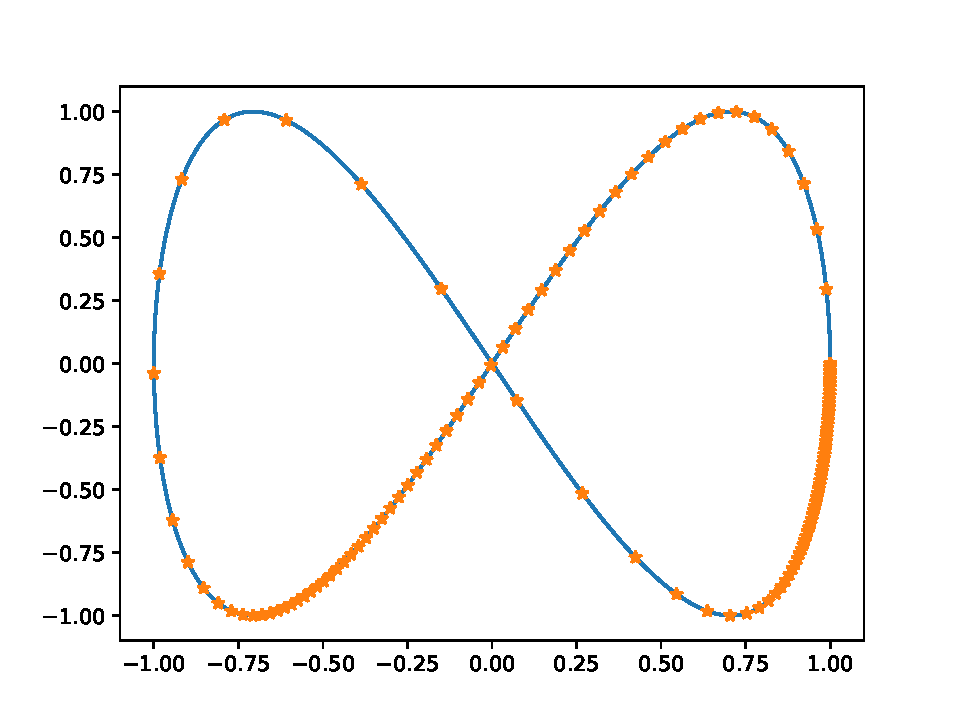
\includegraphics[width=\linewidth]{figures/curve_1/curve_c_1.pdf}
    %     \caption{\(c_1\)}
    % \end{subfigure}
    % \begin{subfigure}[b]{0.5\textwidth}\label{fig:curve_1_c_2}
    %     \centering
    %     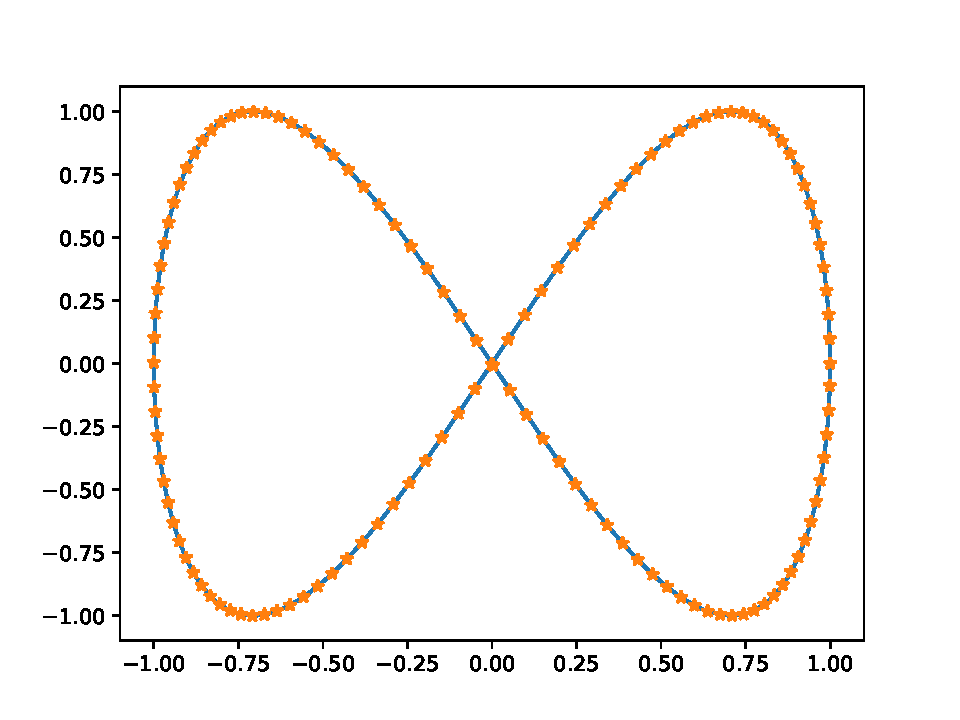
\includegraphics[width=\linewidth]{figures/curve_1/curve_c_2.pdf}
    %     \caption{\(c_2\)}
    % \end{subfigure}
    \begin{subfigure}[t]{0.5\textwidth}
        \centering
        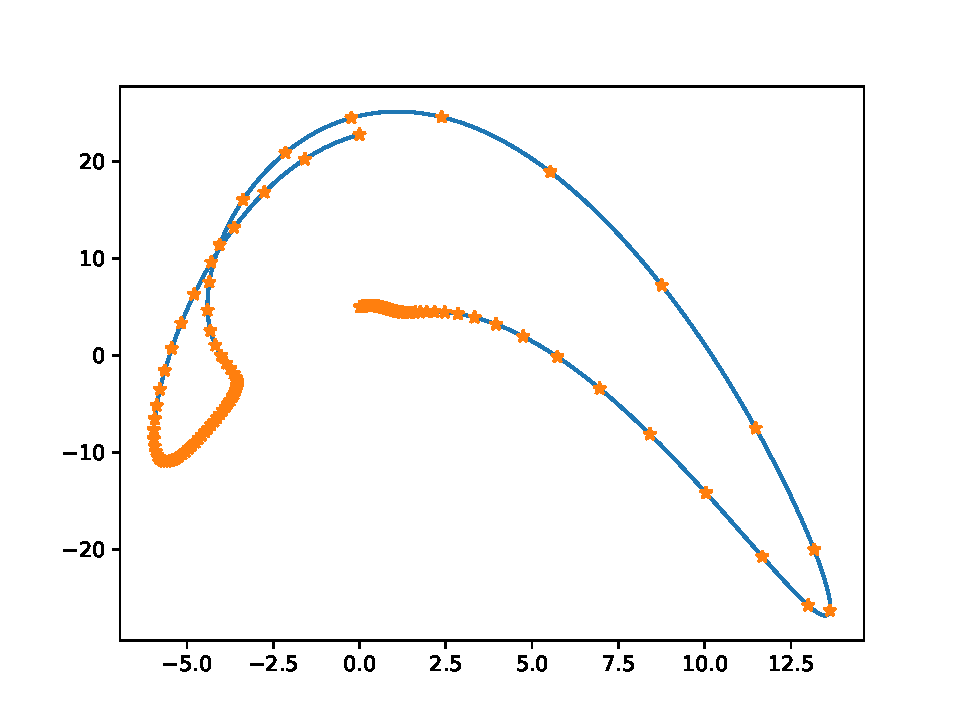
\includegraphics[width=\linewidth]{figures/curve_1/curve_q.pdf}
        \caption{\(q\)}\label{fig:curve_1_q}
    \end{subfigure}
    \begin{subfigure}[t]{0.5\textwidth}
        \centering
        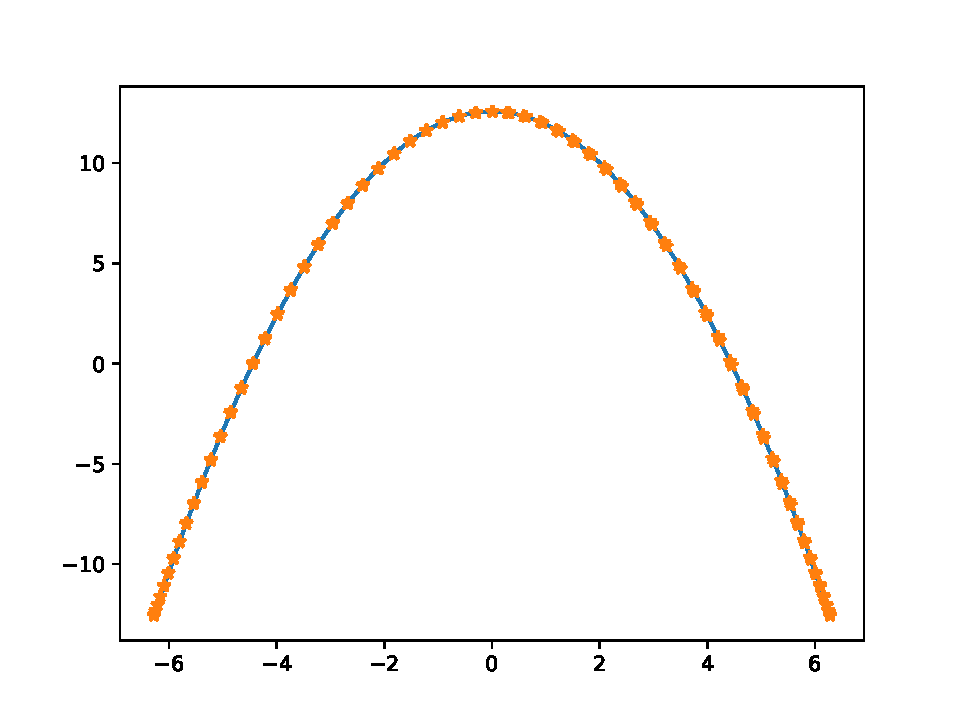
\includegraphics[width=\linewidth]{figures/curve_1/curve_r.pdf}
        \caption{\(r\)}\label{fig:curve_1_r}
    \end{subfigure}
    \caption{The trajectories of \(q\) and \(r\) which are the SRV form defined by the problem in Subsection \ref{subsec:case_1}}\label{fig:curve_1}
\end{figure}


\begin{figure}
    \begin{subfigure}[t]{0.5\textwidth}
        \centering
        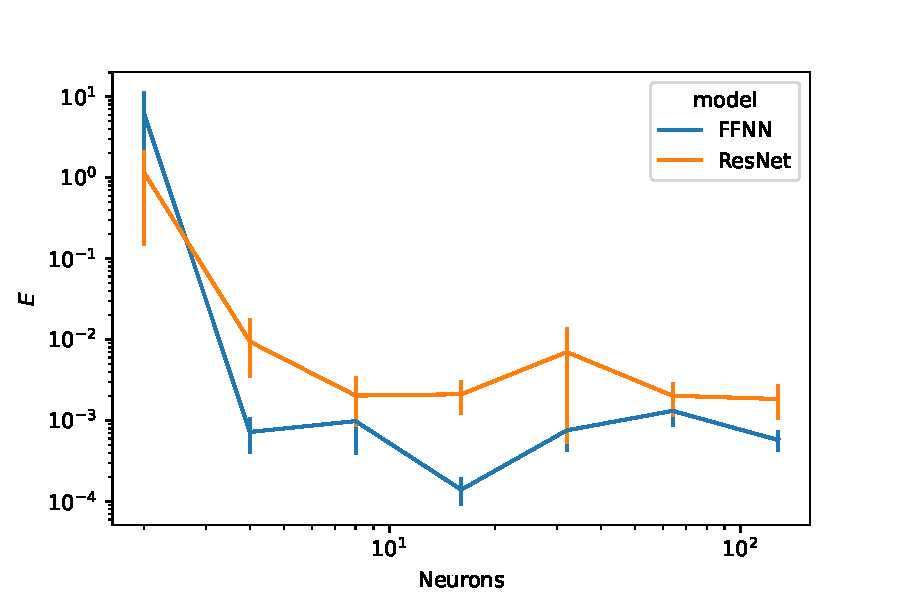
\includegraphics[width=\linewidth]{figures/curve_1/eks_7/neurons_error.pdf}
        \caption{The final cost \(E\) with the number of neurons in each hidden layer.} \label{fig:curve_1_neuron_error} \end{subfigure}
    \begin{subfigure}[t]{0.5\textwidth}
        \centering
        \includegraphics[width=\linewidth]{figures/curve_1/eks_7/layer_error.pdf}
        \caption{Final cost \(E\) with the number of hidden layers.} \label{fig:curve_1_layer_error}
    \end{subfigure}
    \caption{Result of ensemble training with different number of neurons and hidden layers. In Figure \ref{fig:curve_1_neuron_error} the number of layers was fixed at 2. In Figure \ref{fig:curve_1_layer_error} the number of neurons is fixed at 8 per hidden layer. The error bars denote a 80\% confidence interval found by bootstrapping.} \label{fig:curve_1_parmas_eks}
\end{figure}

\begin{figure}[b]
    \begin{subfigure}[t]{0.5\textwidth}
        \centering
        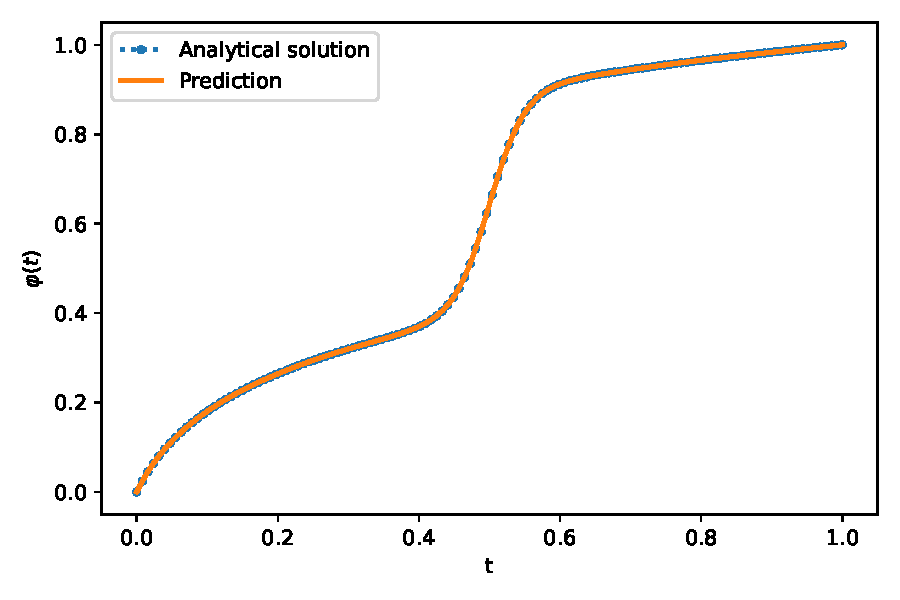
\includegraphics[width=\linewidth]{figures/curve_1/eks_7/plot_2_0.pdf}
        \caption{The approximate optimal reparametrization and the analytical solution.}\label{fig:curve_1_solution}
    \end{subfigure}
    \begin{subfigure}[t]{0.5\textwidth}
        \centering
        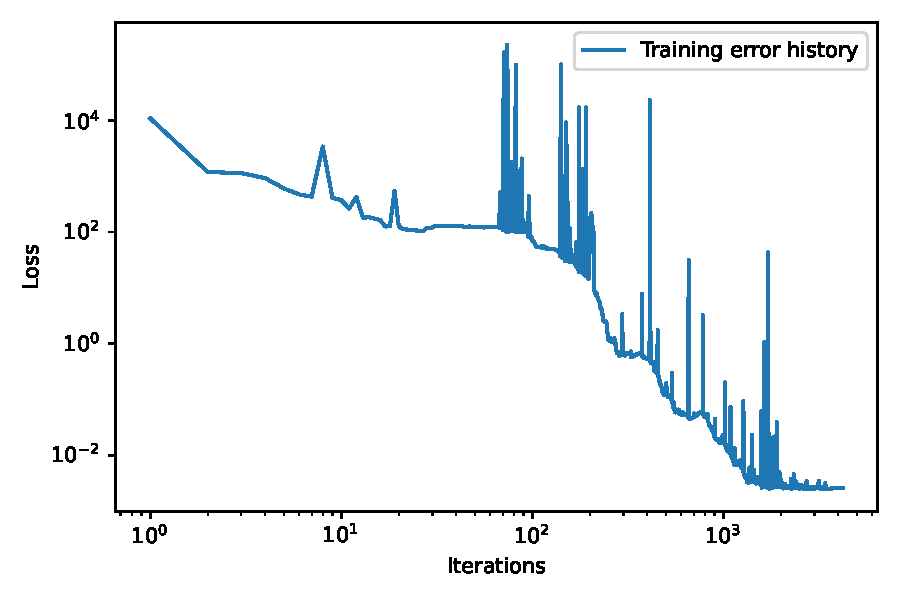
\includegraphics[width=\linewidth]{figures/curve_1/eks_7/history_plot_2.pdf}
        \caption{The cost function \(\mathcal{J}(\theta)\) with each iteration.}\label{fig:curve_1_history}
    \end{subfigure}
    \caption{Result of one optimization procedure with the corresponding loss history.}\label{fig:curve_1_example}
\end{figure}


We performed ensemble training with different network structures, lengths, and widths to test how our method performs on the problem. An overview of the result is shown in Figure \ref{fig:curve_1_parmas_eks}. Moreover, the resulting optimal reparametrization of the first training procedure can be seen in Figure \ref{fig:curve_1_example}. One possible observation is that a ResNet structure permits the training of deeper neural networks better than fully connected feedforward networks.

Reparametrization by neural networks was also compared to deep reparametrization. The comparison was made with respect to the cost function \(\hat E\), as defined in \eqref{eq:discretized_cost}, and is shown in Table \ref{tab:comare_res_palais}. We see that deep reparametrization outperforms our method significantly for this problem. Moreover, deep reparametrization produced the same solution for each training. This is not the case for reparametrization by neural networks since the initial condition \(\theta_0\) is random.
\begin{table}[b]
    \centering
    \begin{tabular}{lrl}
        \toprule
        \(\hat{E} \) & Degrees of freedom & Model         \\
        \midrule
        0.002212     & 33                 & ResNet        \\
        0.000676     & 2257               & ResNet        \\
        0.004567     & 30                 & Deep reparametrization \\
        0.000002     & 10000              & Deep reparametrization\\
        \bottomrule
    \end{tabular}
    \caption{Comparison of the performance of reparametrization by residual neural network and deep reparametrization. Each experiment is the average of the same optimization procedure. Deep reparametrization was performed using. Here the degrees is meant as the number of trainable parameters in the model.}\label{tab:comare_res_palais}
\end{table}


\FloatBarrier
\subsection{Curves from different shapes}
\begin{figure}[t]\label{fig:curve_2}
    \begin{subfigure}[b]{0.5\textwidth}\label{fig:curve_2_c_1}
        \centering
        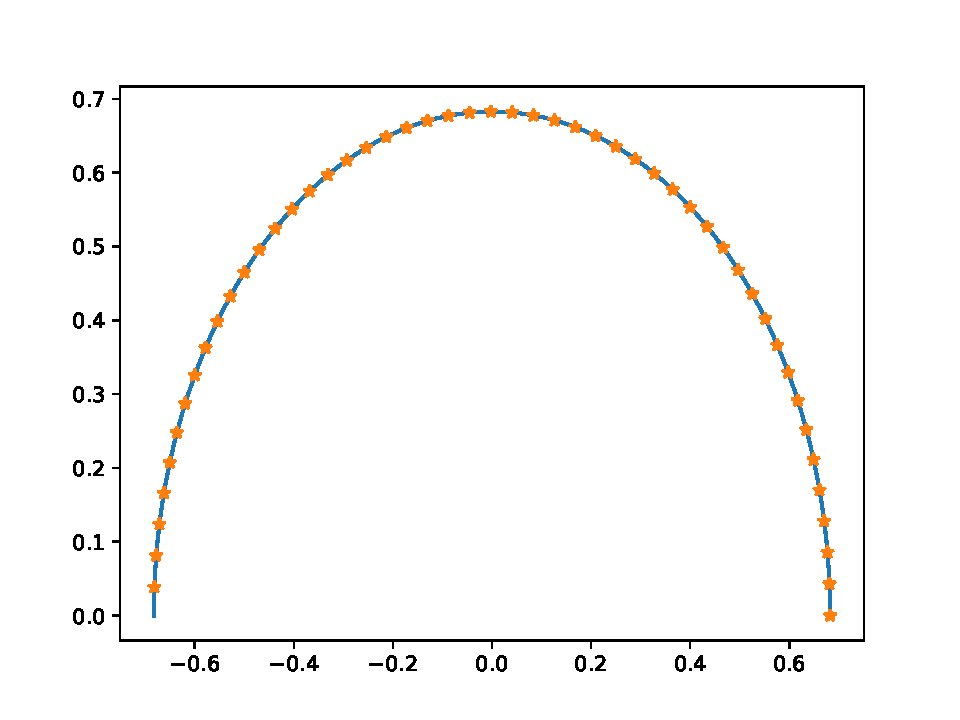
\includegraphics[width=\linewidth]{figures/curve_2/curve_c_1.pdf}
        \caption{\(c_1\)}
    \end{subfigure}
    \begin{subfigure}[b]{0.5\textwidth}\label{fig:curve_2_c_2}
        \centering
        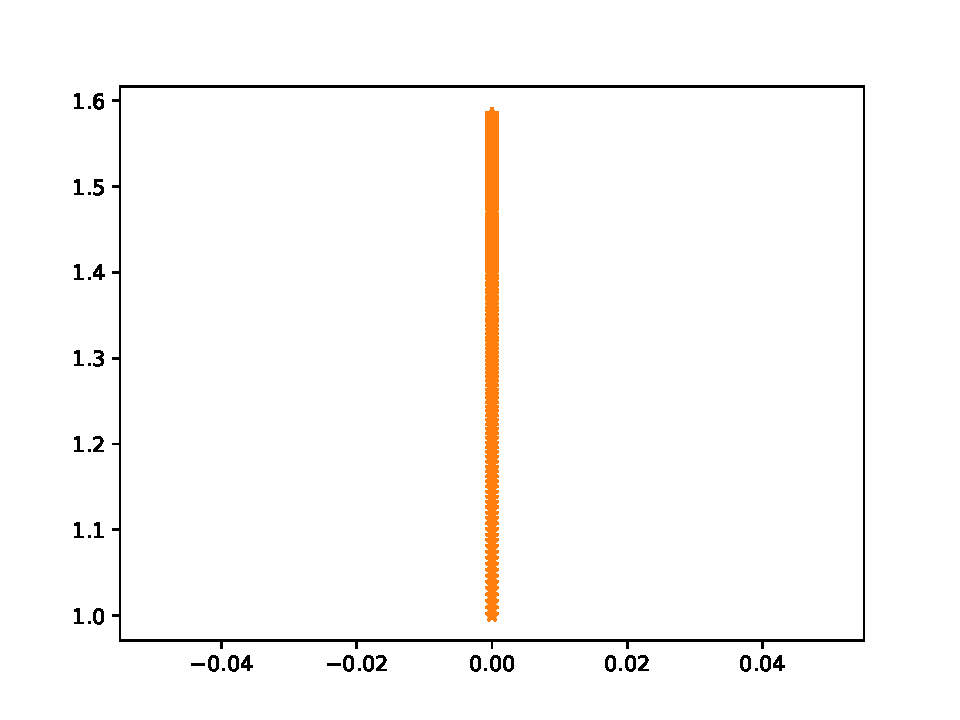
\includegraphics[width=\linewidth]{figures/curve_2/curve_c_2.pdf}
        \caption{\(c_2\)}
    \end{subfigure}
    \begin{subfigure}[t]{0.5\textwidth}\label{fig:curve_2_q}
        \centering
        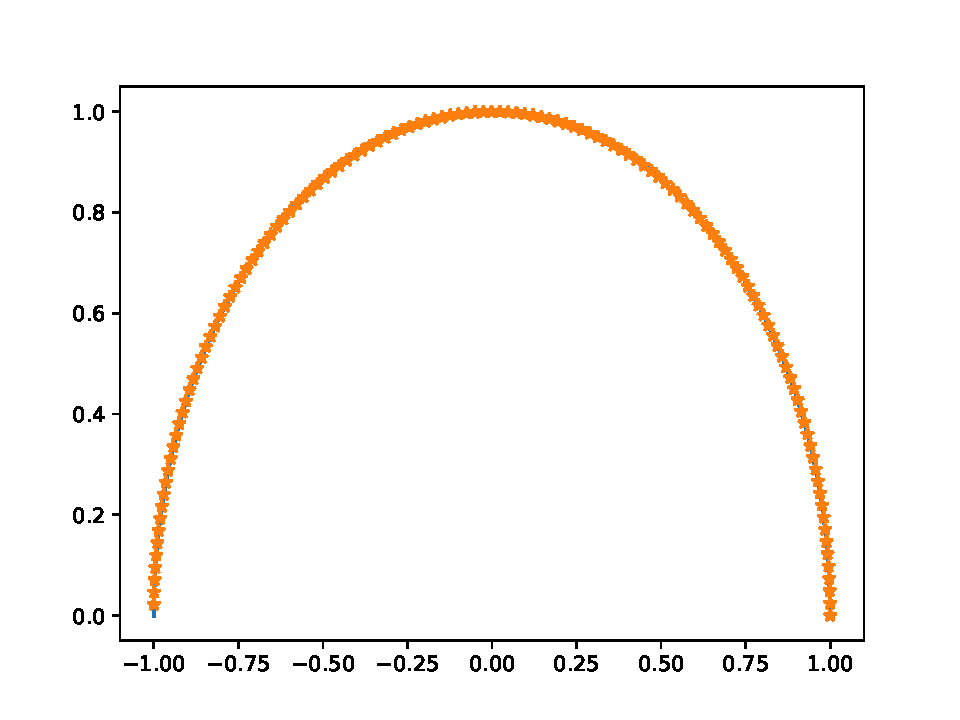
\includegraphics[width=\linewidth]{figures/curve_2/curve_q.pdf}
        \caption{\(q\)}
    \end{subfigure}
    \begin{subfigure}[t]{0.5\textwidth}\label{fig:curve_2_r}
        \centering
        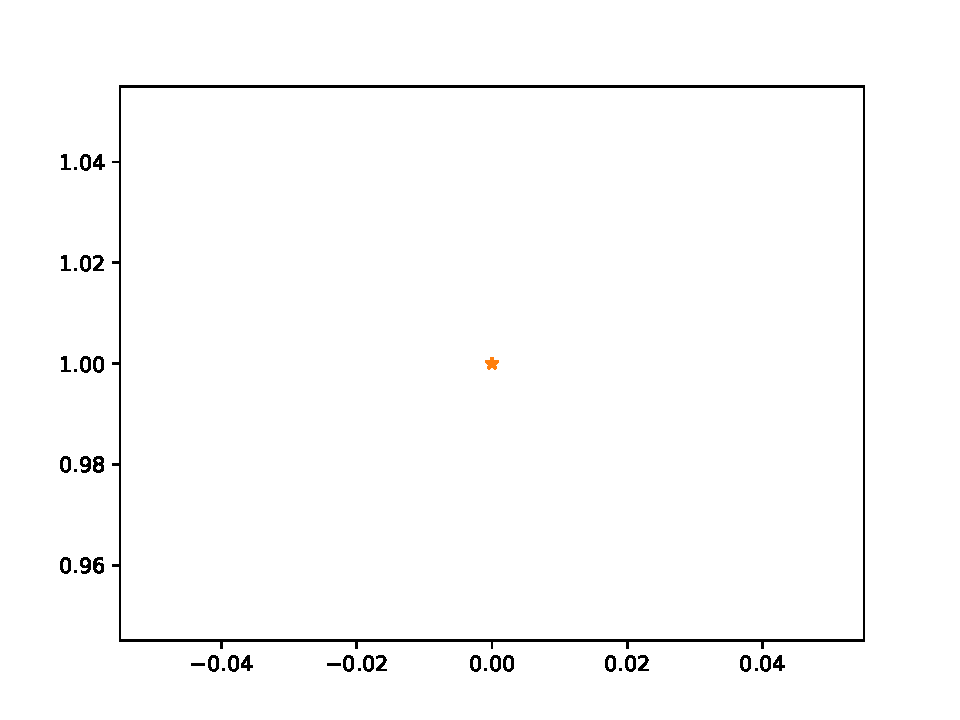
\includegraphics[width=\linewidth]{figures/curve_2/curve_r.pdf}
        \caption{\(r\)}
    \end{subfigure}
    \caption{The trajectory of \(c_1, c_2 \in \text{Imm}(I, \R^2)\), \(q = Q(c_1)\) and \(r = Q(c_2)\).}
\end{figure}

\begin{figure}[t]\label{fig:curve_2_example}
    \begin{subfigure}[t]{0.5\textwidth}\label{fig:curve_2_solution}
        \centering
        \includegraphics[width=\linewidth]{figures/curve_2/curve_2_exp_2/curve_2_exp_2_1_0.pdf}
        \caption{The approximate optimal reparametrization and the analytical solution.}
    \end{subfigure}
    \begin{subfigure}[t]{0.5\textwidth}\label{fig:curve_2_history}
        \centering
        \includegraphics[width=\linewidth]{figures/curve_2/curve_2_exp_2/history_curve_2_exp_2_0.pdf}
        \caption{The cost function \(L(\theta)\) with each iteration.}
    \end{subfigure}
    \caption{The approximate solution to test problem (2) found by a neural network and the corresponding loss history.}
\end{figure}

\begin{figure}[t]\label{fig:curve_2_parmas_eks}
    \begin{subfigure}[t]{0.5\textwidth}
        \centering
        \includegraphics[width=\linewidth]{figures/curve_2/curve_2_exp_2/neurons_error.pdf}
        \caption{The final cost \(E\) with the number of neurons in each hidden layer.}
        \label{fig:curve_2_neuron_error}
    \end{subfigure}
    \begin{subfigure}[t]{0.5\textwidth}
        \centering
        \includegraphics[width=\linewidth]{figures/curve_2/curve_2_exp_2/layer_error.pdf}
        \caption{Final cost \(E\) with the number of layers.}
        \label{fig:curve_2_layer_error}
    \end{subfigure}
    \caption{Result of ensemble training for test problem (2) with different number of neurons and hidden layers. In Figure \ref{fig:curve_2_neuron_error} the number of layers was fixed at 2. In Figure \ref{fig:curve_2_layer_error} the number of neurons is fixed at 8 per hidden layer. The error bars denote a 80\% confidence interval found by bootstrapping.}
\end{figure}


Better structures and optimization algoritmhs for deeper networks.


\FloatBarrier
\subsection{Piecewise linear and piecewise constant}

\begin{figure}[t]\label{fig:curve_1_pc}
    \begin{subfigure}[t]{0.5\textwidth}\label{fig:curve_1_pc_q}
        \centering
        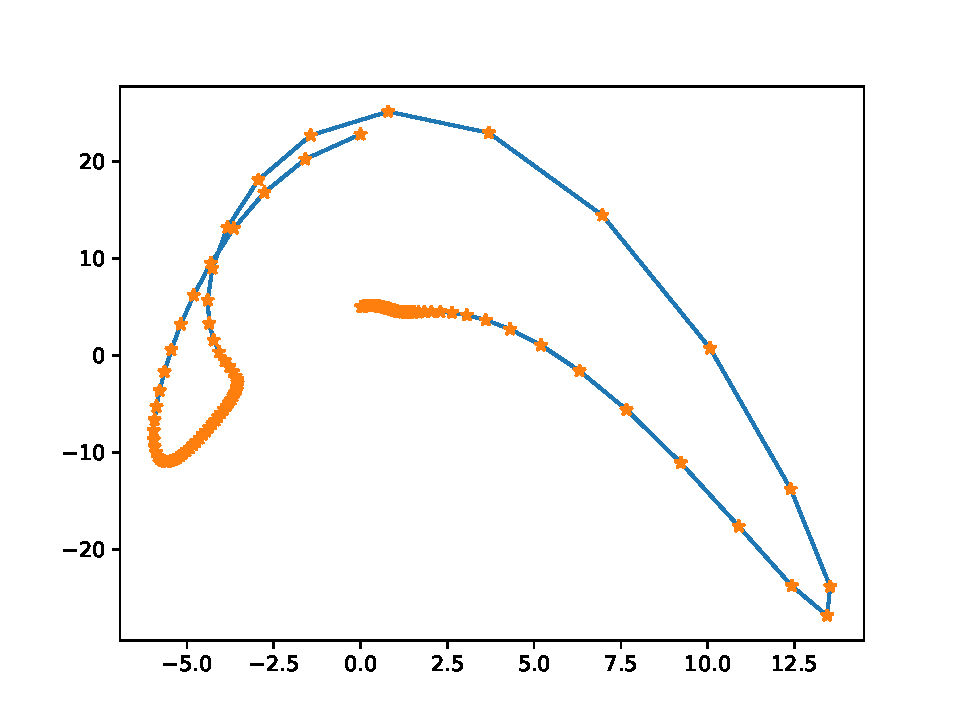
\includegraphics[width=\linewidth]{figures/curve_1/curve_q_pc.pdf}
        \caption{\(\bar q\)}
    \end{subfigure}
    \begin{subfigure}[t]{0.5\textwidth}\label{fig:curve_1_pc_r}
        \centering
        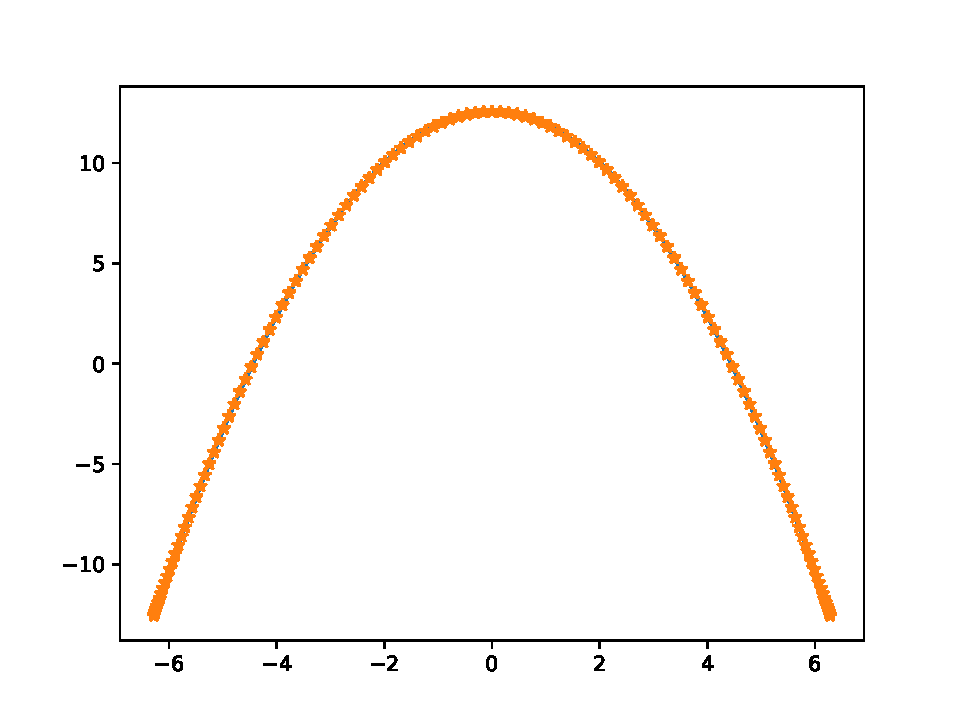
\includegraphics[width=\linewidth]{figures/curve_1/curve_r_pc.pdf}
        \caption{\(\bar r\)}
    \end{subfigure}
    \caption{The trajectory of \(\bar q\) and \(\bar r\) being piecewise constant interpolations of $q$ and $r$ from test problem (1).}
\end{figure}

\begin{figure}[t]\label{fig:curve_1_pc_pl_example}
    \begin{subfigure}[t]{0.5\textwidth}
        \centering
        \includegraphics[width=\linewidth]{figures/curve_1_pc/curve_pc_1/curve_pc_1_0_0.pdf}
        \caption{The approximate optimal reparametrization and the analytical solution.}
        \label{fig:curve_1_pc_solution}
    \end{subfigure}
    \begin{subfigure}[t]{0.5\textwidth}
        \centering
        \includegraphics[width=\linewidth]{figures/curve_1_pc/curve_pc_1/history_curve_pc_1_0.pdf}
        \caption{The cost function \(L(\theta)\) with each iteration.}
        \label{fig:curve_1_pc_history}
    \end{subfigure}
    \begin{subfigure}[t]{0.5\textwidth}
        \centering
        \includegraphics[width=\linewidth]{figures/curve_1_pl/curve_1_pl_exp_1/curve_1_pl_exp_1_1_0.pdf}
        \caption{The approximate optimal reparametrization and the analytical solution.}
        \label{fig:curve_1_pl_solution}
    \end{subfigure}
    \begin{subfigure}[t]{0.5\textwidth}
        \centering
        \includegraphics[width=\linewidth]{figures/curve_1_pl/curve_1_pl_exp_1/history_curve_1_pl_exp_1_1.pdf}
        \caption{The cost function \(L(\theta)\) with each iteration.}
        \label{fig:curve_1_pl_history}
    \end{subfigure}
    \caption{The approximate solutions to the piecewise constant (\ref{fig:curve_1_pc_solution}) and piecewise linear (\ref{fig:curve_1_pl_solution}) version of test problem (1). The approximate solution is compared to the analytical solution of test problem (1) and the corresponding training history is shown in the figure to the right.}
\end{figure}

\begin{figure}[t]\label{fig:curve_1_pl_eks}
    \begin{subfigure}[t]{0.5\textwidth}
        \centering
        \includegraphics[width=\linewidth]{figures/curve_1_pl/curve_1_pl_exp_1/neurons_error.pdf}
        \caption{The final cost \(E\) with the number of neurons in each hidden layer.}
        \label{fig:curve_1_pl_neuron_error}
    \end{subfigure}
    \begin{subfigure}[t]{0.5\textwidth}
        \centering
        \includegraphics[width=\linewidth]{figures/curve_1_pl/curve_1_pl_exp_1/layer_error.pdf}
        \caption{Final cost \(E\) with the number of layers.}
        \label{fig:curve_1_pl_layer_error}
    \end{subfigure}
    \caption{Result of ensemble training for the piecewise linear version of test problem (1) with different number of neurons and hidden layers. In Figure \ref{fig:curve_2_neuron_error} the number of layers was fixed at 2. In Figure \ref{fig:curve_2_layer_error} the number of neurons is fixed at 8 per hidden layer. The error bars denote a 80\% confidence interval found by bootstrapping.}
\end{figure}

Training of
Error convergence example 

\FloatBarrier
\subsection{Interpolated motion capture data}
In the following experiments, we used two motions from the CMU Graphics Lab Motion Capture Database \cite{mocap}. As seen in subsection \ref{subsec:shape-lie}, motion capture data can be interpolated such that the SRV form is piecewise constant. As in the previous section, these SRV curves were then interpolated by a piecewise linear interpolation. The interpolated curves were then used instead of the original curves in the optimization procedure. As seen in Figure \ref{fig:curve_1_so3_example} the interpolated problem produced an in optimal reparametrization that agreed with the solution given by dynamic programming, implemented by \citeauthor{lystad2019}\cite{lystad2019}. 

\begin{figure}[t]
    \begin{subfigure}[t]{0.5\textwidth}
        \centering
        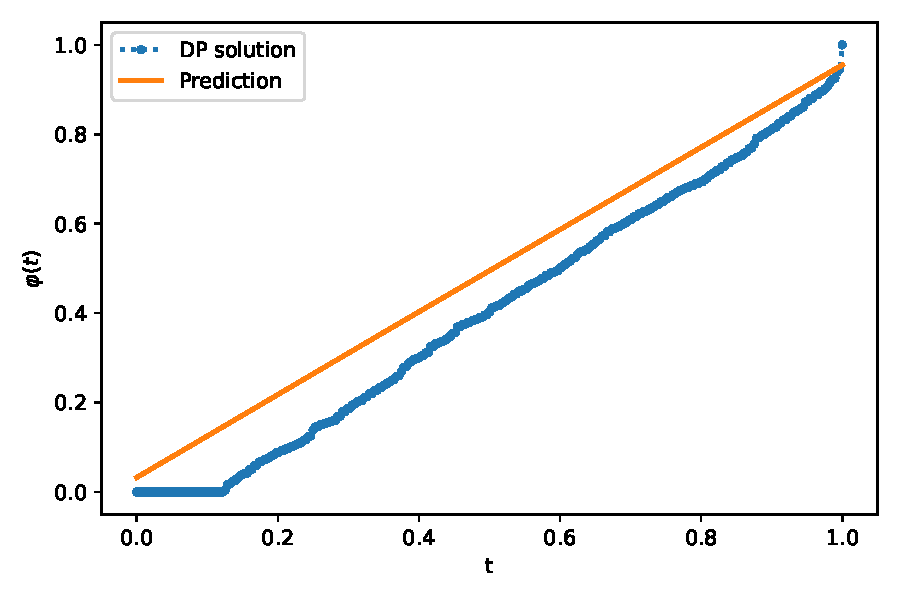
\includegraphics[width=\linewidth]{figures/curve_so3/pc_eks_2/plot_1_0.pdf}
        \caption{Solutions found by neural network training and dynamic programming.}\label{fig:curve_so3_pc_solution}
    \end{subfigure}a
    \begin{subfigure}[t]{0.5\textwidth}
        \centering
        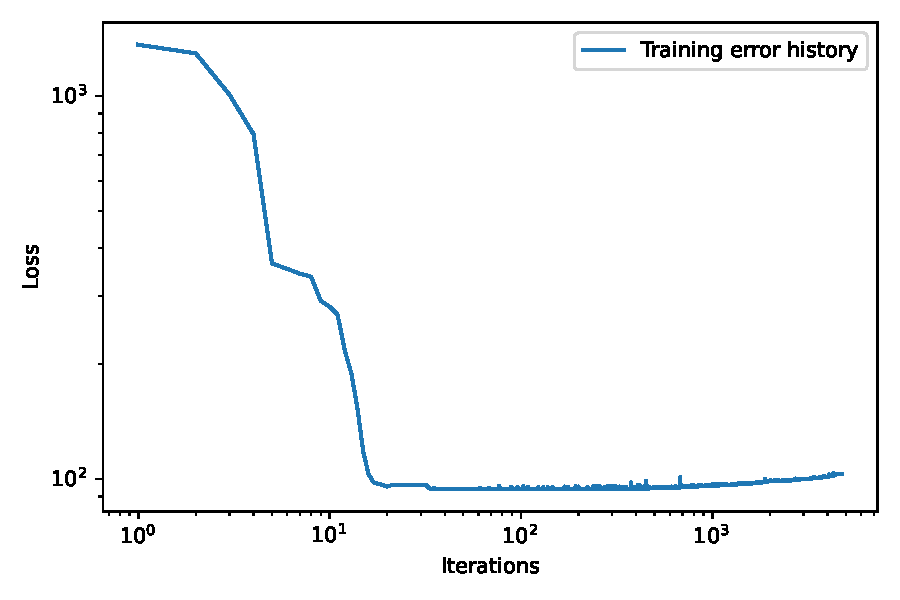
\includegraphics[width=\linewidth]{figures/curve_so3/pc_eks_2/history_plot_1.pdf}
        \caption{The cost function \(L(\theta)\) with each iteration.}\label{fig:curve_so3_pc_history}
    \end{subfigure}
    \begin{subfigure}[t]{0.5\textwidth}
        \centering
        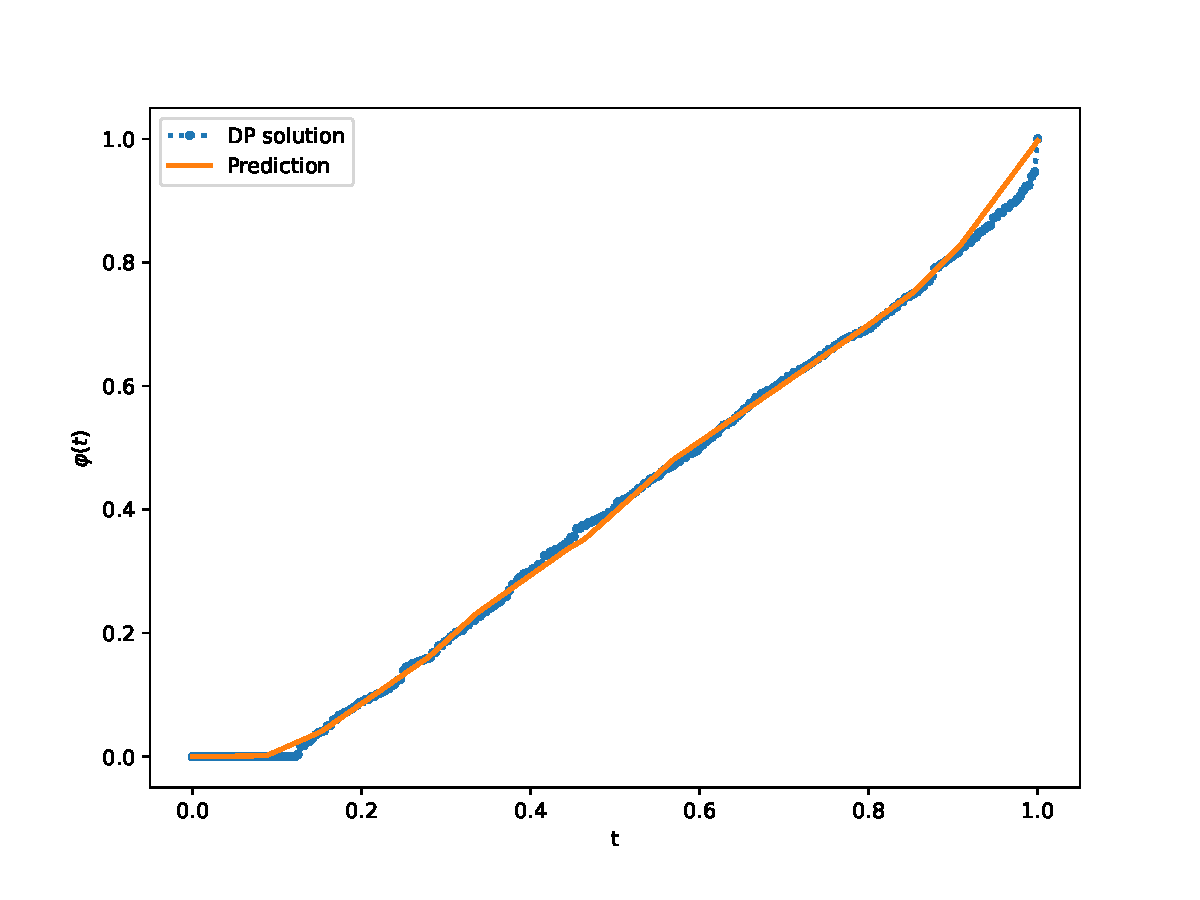
\includegraphics[width=\linewidth]{figures/curve_so3/pl_eks_6/plot_288_0.pdf}
        \caption{Solutions found by neural network training and dynamic programming.}\label{fig:curve_so3_pl_solution}
    \end{subfigure}
    \begin{subfigure}[t]{0.5\textwidth}
        \centering
        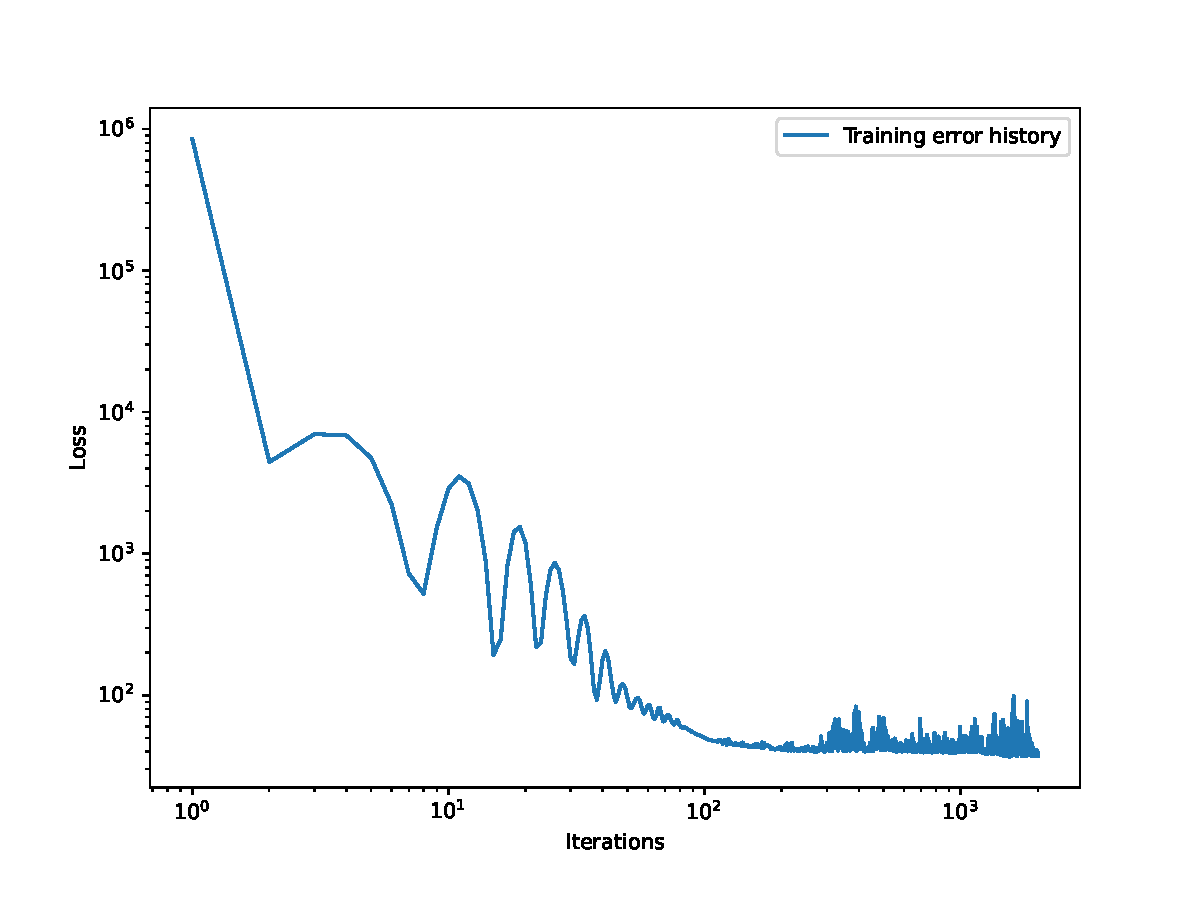
\includegraphics[width=\linewidth]{figures/curve_so3/pl_eks_6/history_plot_288.pdf}
        \caption{The cost function \(L(\theta)\) with each iteration.}\label{fig:curve_so3_pl_history}
    \end{subfigure}
    \caption{The approximate optimal reparametrizations of two curves representing motion capture data. Figure \ref{fig:curve_so3_pc_solution} shows the solution for the original curves, and Figure \ref{fig:curve_so3_pl_solution} shows the solution for the linearly interpolated curve. The approximate solutions are compared to the solution found by a dynamic programming algorithm and the corresponding training history is shown in the figure to the right. }\label{fig:curve_1_so3_example}
\end{figure}

Ensemble training was again performed to observe how the optimal reparametrization is affected by different parameters. The ensemble training result is shown in Figure \ref{fig:curve_so3_pl_eks}. In this experiment, the network structure was not varied. Instead, the performance of ReLU and \(\tanh\) activation function was compared. 

\begin{figure}[t]
    \begin{subfigure}[t]{0.5\textwidth}
        \centering
        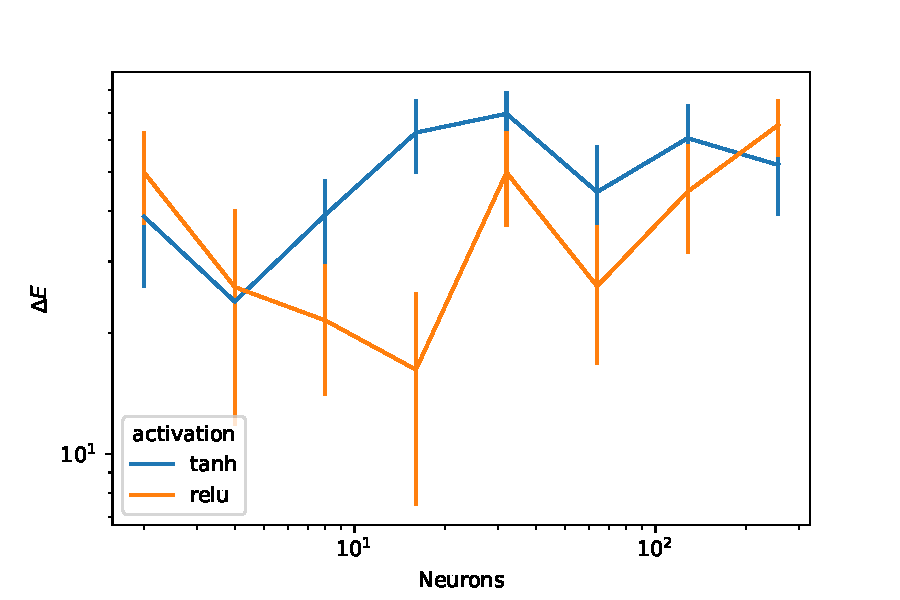
\includegraphics[width=\linewidth]{figures/curve_so3/pl_eks_6/neurons_error.pdf}
        \caption{The final cost \(E\) with the number of neurons in each hidden layer.}\label{fig:curve_so3_pl_neuron_error}
    \end{subfigure}
    \begin{subfigure}[t]{0.5\textwidth}
        \centering
        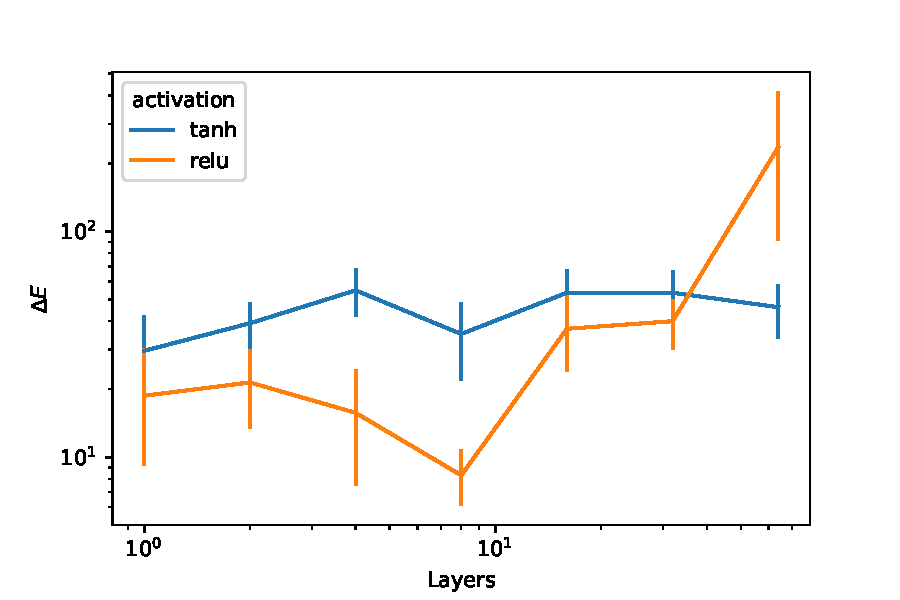
\includegraphics[width=\linewidth]{figures/curve_so3/pl_eks_6/layer_error.pdf}
        \caption{Final cost \(E\) with the number of layers.}\label{fig:curve_so3_pl_layer_error}
    \end{subfigure}
    \caption{Result of ensemble training for the piecewise linear version of the problem with curves generated by motion capture data with different number of neurons and hidden layers. Figure \ref{fig:curve_2_neuron_error} the number of layers was fixed at 2. In Figure \ref{fig:curve_2_layer_error} the number of neurons is fixed at 8 per hidden layer. The error bars denote a 80\% confidence interval found by bootstrapping.}\label{fig:curve_so3_pl_eks}
\end{figure}



\section{Conclusion}

\section*{Appendix}
The code for this project can be found at \url{https://github.com/alexarntzen/prosjektoppgave}
Motion capture by 
\cite{mocap}
\printbibliography
\end{document}

